

\subsection{DeepmindLab navigation challenge}
We propose a 5-stage benchmark for reinforcement learning based methods to address the navigation problem.
While there already exists optimal algorithms to find shortest path between two points and perform optimal navigation between given set of points in a given map, the advantage of Deep reinforcement learning comes from it's ability to extract required features from the input images.
Thus we need to either integrate existing path planning and mapping methods with deep learning methods to perform end-to-end training or extend deep learning methods to learn path planning and mapping.
As we have shown this is going to be hard.
\begin{description}
  \item[Evaluate on training map with fixed goal location]
    This is the textbook version of reinforcement learning problem,
    especially in gridworld. This problem is easier because the policy
    is stationary at the train time and does not changes during
    testing.
    We propose the evaluation metric to be : the time taken to hit the goal once. We show the results on this benchmark in Table~\ref{tab:TODO-RUNEXP}.
    We compare the results against optimal planning methods which take the support of external map input.
  \item [Evaluate on training maps with random goal location]
    Solving this problem through Reinforcement learning is harder becuase the policy function needs to depend up on the goal location.
    This problem is attempted by \cite{MiPaViICLR2017} with limited success.
    As their experiments and confirmed by our experiments, the navigation strategy learnt by the agent is nowhere near optimal.
    So instead of learning a static policy function the learning algorithm needs to learn a function that returns a different policy for different goal locations.
    This can be evaluated into ways, (a) providing the goal location as an external input to the method or (b) let the agent explore the map randomly and ask the agent to return to goal location after first round of exploration.
    We chose method (b) and show our results on this in Table~\ref{tab:TODO}.
    We compare the method against random systematic explorers, where the agent always moves forward and takes right turns on all junctions.
  \item [Evaluate on unseen maps]
    Any proposed algorithms on navigation problems, should be evaluated on unseen maps.
    Since this is a hard problem, we should compare it against random systematic explorers and should be analyzed to understand the kind of approach the learning algorithm is using.
    \begin{description}
      \item[Remember and repeat]
        We propose a series of maps, goal and spawn locations where the optimal performance can be achieved by repeating the action sequence that lead to the goal for the first time.
      \item[Frame to action mapping]
        We propose a series of maps, goal and spawn locations where the optimal performance can be achieved by learning a frame to action greedy mapping but not just by remember and repeat.
      \item[Full path planning]
        We propose a series of maps, goal and spawn locations, where the optimal performance cannot be achieved unless full path planning is done.
    \end{description}
\end{description}

\begin{figure}%
 \vspace{-3em}%
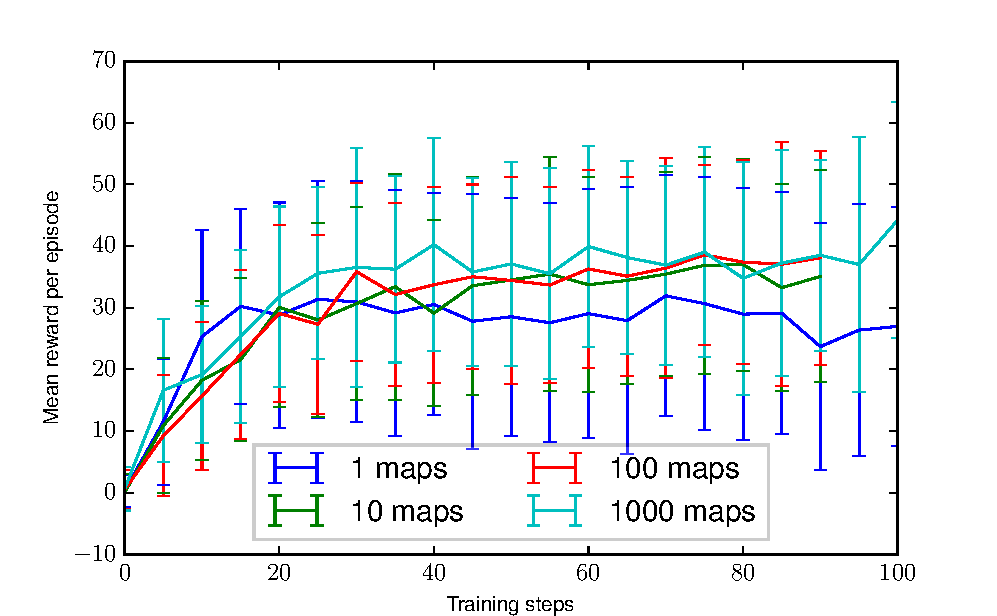
\includegraphics[width=0.5\columnwidth]{images/plot_reward_3D-1000.pdf}%
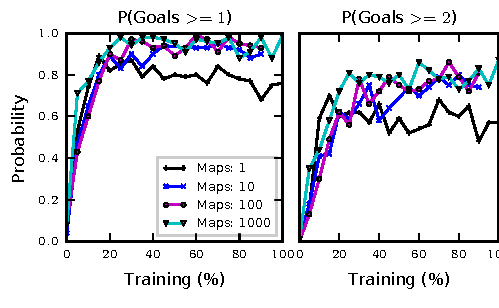
\includegraphics[width=0.5\columnwidth]{images/plot_probability_3D-1000.pdf}%
\vspace{-1em}%
\caption{Mean reward while tested on 100 unseen maps, while being trained on different number of training maps. Note that while training on 1000 maps eventually achieves high reward, it is only higher mean reward (44.2), training on 1 map hits the maximum (31) much faster.}%
\label{fig:plot_reward_on_testing}%
\end{figure}
